
\chapter{Spark ignition engine}
\section{Mixture preparation in SI engine}
	\wrapfig{6}{l}{5}{0.25}{ch4/1}{ch4/1}
	The objective is to obtain an homogeneous gaseous composition with the right equivalence ratio. We will see that in direct injection inhomogeneous gas is obtained. 
	
\subsection{The carburetor}
	It is now outdated because of the regulation imposed on the exhaust gases and has been replaced by fuel injection except\ \\
	 
	\wrapfig{4}{r}{5}{0.35}{ch4/2}{ch4/2}
	for small engines.  As a first approximation we can consider that the carburetor pump the fuel into the air flow using the Bernouilli principle (compressible): when the air velocity increases the static pressure decreases and the fuel flow increases. 
	
\subsubsection{Importance of equivalence ratio for combustion}
	\wrapfig{7}{l}{4}{0.5}{ch4/3}{ch4/3}
	The best burning condition is obtained when stoechiometry (15kg air for 1kg fuel). But rich and lean mixture can also burn not in the best conditions. In SI engine the amount of mixture going to the engine is controlled by the throttle. A venturi creates a decrease in pressure for the fuel to be pushed.  
		
	\ \\
	
	\wrapfig{7}{r}{6}{0.3}{ch4/4}{ch4/4}
	The reality deviates from the incompressible model. Indeed, for air velocity increase the pressure drop is more important and the injected fuel is larger as fuel is incompressible (eq. ratio higher in high air flow). In addition the speed in venturi is limited to Mach 1 to avoid shocks and the fuel height pressure has to be compensated in order to have injection, thus for low speeds there is no injection. 
	\newpage

\subsubsection{Compensating jet}
	\wrapfig{8}{l}{5}{0.3}{ch4/5}{ch4/5}
	This is introduced in order to solve the problem of the increasing equivalence coefficient when air flow increases. The fuel jet is divided into 2 jets, the main directly connected to the venturi and the second connected to the venturi through an \textbf{emulsion tube}. As the air flow increases, the one into the emulsion tube too and this decreases the amount of compensating fuel. 
	
	\ \\\\
	
	\wrapfig{6}{r}{4}{0.3}{ch4/6}{ch4/6}
	Here we can see the effect of this, we have a more constant eq. ratio. As we have decrease the flow of the main jet and the compensating jet is not working at high air speed, the mixture is kept constant. When acceleration, rich mixture is needed. For this an additional system sensing the acceleration provides extra fuel. 
	
\subsubsection{Idling fuel line}
	\minifig{ch4/7}{ch4/8}{0.35}{0.35}{0.3}{0.3}
	The remaining problem is at very low air flow rate because the pressure drop at the venturi is very low. To compensate this, one takes advantage from the flow near the throttle where a local pressure drop is created when nearly closed and uses so the \textbf{idling fuel line}.  The last trick to include is for \textbf{cold start}. The added \textbf{choke valve} is situated before the venturi in order to create a choke. 
	
\subsection{Fuel injection}
	\minifig{ch4/9}{ch4/10}{0.35}{0.35}{0.45}{0.4}
	The advantages of fuel injection with regard to the carburator is listed above. 
	
	\wrapfig{8}{l}{6}{0.3}{ch4/11}{ch4/11}
	The injection is not linked to the air flow, we need thus a control unit in order to control the injection. In the industry, electronic is used for the Engine Control Unit (ECU) based on the input of many sensors, direct or indirect measurement of air flow. 
	
\subsubsection{Direct injection}
	Even if it is more complex, it allows better volumetric efficiency: the fuel is evaporated after injection and thus decreases the air density in the mixture, thus we can intake air at higher load (the cooling is better). In addition, the load is stratified and allow more efficient intake since losses are decreased: lean mixture can be formed and then managed in the piston. 
	
\subsubsection{Preparation strategies}
	\wrapfig{8}{r}{7}{0.3}{ch4/12}{ch4/12}
	There are 3 main categories of guiding the injected fuel to the spark plug: wall-guided, air-guided and spray-guided. The wall-guided consist in using the wall of the piston to get the best mixture, there is for example a small hole. As introduced, it is possible with direct injection to intake inhomogeneous mixture. But we still need an equivalence ratio of 1 for good combustion. To get this condition near the spark plug, the flow conditions can be changed $\rightarrow$ air-guided. 
	
	\ \\
	The disadvantages of the wall-guided is that it requires good flow conditions and good injection timing, reducing the advantage of improved volumetric efficiency. In addition it is bad for emission. The most efficient but also most complex system is the spray-guided. It relies on the high pressure (no need of high air speed in the chamber) and fast response of the injector to obtain the adequate mixture without interaction with the wall, hence avoiding wall wetting (less emission).  The mixture is more homogeneous. 
	
\section{Ignition}
	The task of the ignition devices are to: 
	\begin{itemize}
	\item[•] In practice, the ignition is not instanteneous and thus we need to introduce an advance delay for the spark ignition. 

 	\item[•] 	In the chamber we have certain pressure, certain temperature, we have to deliver a high voltage in order to create the spark. 

	\item[•]	Depending on the layout we have to distribute the spark, if we have a multi-cylinder we have a phase between the different strokes. 
	
	\item[•] We have to provide enough energy as well as power and duration to ignite.  \\
	\end{itemize}

\subsection{Spark production}	
	Previously we performed ignition by current interuption with a breaker in the piston, but the breaker was eroded and we need to replace it. This was done with low voltage, limiting the compression ratio. Now, for high voltage ignition we have: coil, transistor, electronic or magneto ignition. 

\subsubsection{Coil ignition}
	\wrapfig{12}{l}{7}{0.3}{ch4/13}{ch4/13}
	The principle of coil is based on the basic electrical relation $V = L\frac{dI}{dt}$ meaning that we will have a huge voltage if we brake the circuit in the primary, that will be converted to a higher voltage in secondary circuit. The problem was the distance to the plug (have to pass from a distributor) and thus the loss of voltage due to humidity. To solve the problem, the distributor and the coil are placed near the plug. The duration of the spark is short. 
	
	\ \\
	The big problem with the coil circuit is that as we know, after discharge we need to recharge the coil through a resistance, but this takes some times. This is not a problem for normal circuit but for the engine that must deliver the spark at a fixed time to several cylinders it is. This means that the time constant $\tau = L/R$ must be lower than the switching frequency between cylinders: 
	
	\begin{equation}
	f = \frac{Nn}{120}
	\end{equation}
	
	where N is the stroke and n the rotational speed of the engine (caution: we divide by 60 if it is a 2 strokes engine). How to work on the time constant? If we lower L we will have less energy in the inductance, if we increase R, the current is lower. If the n is going to increase we have less time to produce spark. 
	
\subsubsection{Electronic ignition}
\wrapfig{8}{r}{6}{0.2}{ch4/15}{ch4/15}
Today this is used instead of the previous. In the processor we have a number of parameter like rpm, the right position of the crank, etc. We have the exact position on the throttle position. Knocking can also change the pre-ignition angle thus it is also considered. 

\subsection{Voltage requirements}
	The voltage we need to apply (kV) is varying with the mixture, we need less kV for $\lambda = 1$ than for lean or rich mixtures. \\
	
	The kV is also depending on the electrodes distance, if it is enlarged we need more kV and the contrary if the distance is shorter. The problem when shortened is that if some solid deposits form on the plug, the contact would make a short circuit. \\

	\wrapfig{8}{l}{7.5}{0.3}{ch4/14}{ch4/14}
	Another parameter is the compression ratio $\epsilon$. The higher $\epsilon$ the higher the air density and thus the higher the voltage needed. Note that the needed voltage decreases with the rpm because it causes turbulences in the flow of air and thus increase the homogeneity. Too much turbulence is bad. The ignition also depends on the operating conditions. On the figure (a) represents the spark in good condition, (b) in bad condition and (c), (d) are the needed voltage respectively using old and new spark plug. On the figure we have to be careful at start. 
	
\subsection{Pre-ignition}
	According to the theory we should ignite when the piston reaches the top dead center. But the ignition process takes time, we will make it ignite before. The condition we want to respect is to have the flame front in contact with the piston when it reaches the top dead center, because before means applying opposite force and after make lose power. If $v$ is the flame front speed and $L$ the chamber distance: 
	
	\begin{equation}
	T = \frac{v}{L} \qquad \Rightarrow \alpha = \omega T = \frac{n}{60}360\frac{L}{v}
	\end{equation}

Where $\alpha$ is the pre-ignition angle; the crankshaft angle to deal with. We could also say that L depends on the size of the combustion chamber: 

\begin{equation}
L \propto V_c = \frac{V_d }{\epsilon -1 } \qquad \Rightarrow \alpha \propto \frac{n}{60}360\frac{V_d }{\epsilon -1 }\frac{1}{v}
\end{equation}

If we look to this formula the two varying parameter are n and v. That flame speed is not supersonic (deflagration). The most important number in fuel is the RON number, a RON 95 is less resistant to the flame than 98 so in principle we have to change the preignition angle if we change the fuel. Now the pre-ignition angle is computed by the computer when running since the rpm is varying. The pre-ignition angle also depends on the load provided by the throttle since the fuel quantity changes. Note that an ignition map can be produced in test bench and the formula would not be necessary. 

\subsubsection{Leading to knock}
	\wrapfig{10}{l}{7.5}{0.25}{ch4/16}{ch4/16}
	If the pre-ignition angle is too large, as the combustion has more time this leads to higher pressure and temperature, auto ignition can happen. On the figure we can see that when the angle increases, waves appear. Knocks are detected by knock sensors by verifying the frequencies (knock = high frequency). This sensor has to be the closest to the combustion sensor since the high frequencies are more damped (viscous model). The configuration of the engine can also make some cylinder more likely to produce knock. 
	
\subsection{Spark plug}
	\minifig{ch4/17}{ch4/18}{0.23}{0.2}{0.4}{0.4}
	The spark plug is composed of the connector (plug wire), ceramic insulator to isolate from the environment and the electrode. An important property is the self cleaning to avoid short circuit. It depends on the engine load. If we go above the safety margin we will have glow ignition, the temperature in this region is not a problem for the plug but even without the spark the ignition will start by itself, we do not control the ignition anymore. When we have a too low temperature, we have no cleaning and the plug get dirty. So we must be in the right range. 
	
	\ \\
	We manage the time of spark plug heating, we get 100\% high temperature at the bottom and then the other heat are distributed (mostly to the cylinder head, allowing the cooling by air or water in this region). This is managed by playing with the plug shape. 
	
\section{Combustion}
\subsection{The process step by step}
	Let's remind that the combustion is an exothermic chemical oxidation reaction. In SI, the gas is premixed and we ignite it in the chamber. Concerning the type, the normal combustion happens with flame propagation, inducing transport of mass and heat (in laminar or turbulent mixture). If the flame speed is subsonic we speak about deflagration, supersonic = detonation (explosion). Auto-ignition happens without spark under certain temperature and pressure. 
	
\paragraph{Creation of the mixture}
	creation in a carburator or in indirect or direct injection. Consists in evaporated fuel in air (homogeneous and gaseous) at stochiometry 14.7 air for 1 mass fuel. The quality is given by L or $\lambda$ factor: 1 stochiometry, 1.1 minimum consumption, 0.85 power or cold start. 
	
\paragraph{Heating}
	We have some parameter to respect for the preheating of the mixture. We cool the engine in order to avoid auto-ignition and respect aluminum properties, but at regime we should keep a good temperature.  Pre-heating is used for cold start: extracting the air of the exhaust system which is already hot. It is not good to have too hot air since it decreases the density and the capacity in fuel. Recirculation is used because in some cases the fuel is not totally burnt, this allows to cool a bit the exhaust gas too (reduces NOx). Bad for the efficiency. 
	
\paragraph{Compression}
	It will make the temperature rise, pressure too. The heating up to 550\degres C depends on $\lambda$ and $\epsilon$. The higher the compression ratio, the higher the temperature. Is it a fixed value? Normally yes, we can play with it by means of the valves (letting the exhaust open for example). The variable one is interesting since we could increase it when cold start and then decrease it. This also depends on the fuel vaporisation (complete is best). There are various hydrocarbons in fuel and some can make the pressure higher by prereaction. 
	
\paragraph{Ignition}
	The ignition is produced by the spark, the energy needed is very small: 0.5-3 mJ needed while 40 mJ provided. It can be calculated by:

	\begin{equation}
	E _v = cst \frac{d^2}{c}\lambda _m \Delta t
\end{equation}		
	
	where c is the flame speed, d the electrodes distance $\lambda _m$ the conduction and $\Delta T$ the diff between mixture and ignition. For the heat to be good distributed we need high c and $\lambda _m$. After ignition we have a deflagration. 
	
\paragraph{Combustion}
	  \wrapfig{10}{l}{5}{0.3}{ch4/19}{ch4/19}
	  We can see the real curve where there is an ignition lag. Depending on if we are in turbulent or laminar regime we have different flame speed: 
	  
	  \begin{equation}
	  c_l  = f(T)\phi (\lambda)p^{-0.25}\qquad c_t = c_l (1 + \beta c_z ^\alpha \lambda ^\beta p^\gamma)
	  \end{equation}
	
	where $\beta$ is a parameter depending on the shape of the piston and $c_z$ the piston speed. We see that turbulent regime speed is higher. 
	
	\ \\[1cm]
	
\subsection{Influencing parameters}
	\begin{itemize}
	\item[•] \textbf{Thermodynamics:} the fuel, temperature, pressure and $\lambda$ value influences. If $\lambda = 0.87$ we have the highest combustion temperature and combustion speed (rich mixture). 
	\item[•] \textbf{Aerodynamics:} when the rpm increases, the flow is turbulent and the combustion speed increases. 
	\item[•] \textbf{Chemical:} reaction kinetics and propagation mechanism. 
	\item[•] \textbf{Geometrical:} the shape of the piston and combustion chamber can increase turbulence. 
	\item[•] \textbf{Kinematically:} the motion of the piston.
	\end{itemize}
	
\subsection{Abnormal combustion}
	This is a combinaison of normal combustion and auto-ignition, temperature and pressure are very high. Because of the contact between the two flame fronts we have relatively high pressures (waves) and temperatures leading to high frequency vibrations. Piston destruction is possible. 
	
\subsubsection{Influencing parameters}	
	The \textbf{knock} is when the auto-ignition happens after the normal combustion somewhere in the piston. \textbf{Early ignition} happens before the spark. The meeting of the two flame front leads to high pressure and temperature. The influencing parameters: \\
	
	\begin{itemize}
	\item[•] \textbf{Fuel}: the RON number gives an indication on the shock resistance, the molecular structure of the fuel, and some additive as lead (former) and now MTBE. 
	\item[•] \textbf{Properties mixture}:  air/fuel ratio is important since we get the highest temperature with $\lambda = 0.9$, when <1 all fuel does not burn and >1 the air is heated. The inlet temperature is important, higher combustion temperature if inlet hot. The presence of residual gases in the combustion chambers creates irregularities. 
	\item[•] \textbf{Operational parameters}: Rotational speed, if it increases, first of all there is less time to fill the cylinder, so we have less mass to burn the temperature will go down, we create more turbulence, the mixture is better but efficiency decreases (temperature too). If the load increases (full throttle) the temperature increases. We can work on the pre-ignition angle, if we decrease it, we ignite later, we will shift to the dilatation part, the combustion will operate when the expansion. If we make the angle smaller the heat will be lower, the pressure too. This is a process that takes time. 
	\item[•] \textbf{Compression ratio:} if compression ratio rises, t\degres and pressure rises $\Rightarrow$ knock. 
	\item[•] \textbf{Deposits}: on the wall, they decreases the cooling and thus knock. 
	\item[•] \textbf{Shape of the combustion chamber:} play also a role. \\
	\end{itemize}
	
\subsubsection{Glow ignition}
	Glow ignition, the phenomena is the same but the origin is different, if one part is too hot, for example the spark plug should not be above some \degres C, it can ignite without a spark. Same problem with valves and deposits. The characteristics are the same as before for what concerns the effects, the condition too. Outside of the engine we cannot make the difference between the two types of ignition. For deposits, they burn with the knock thus disappear. \\
	
	After-dieseling is the phenomenon when you switch the engine off, it continues to run because deposits are burning (after heavy loading of the engine $\rightarrow$ carbon deposits). 
	
\subsection{Design of the combustion chamber}
	The shape of the combustion chamber is important, the constraints are: avoiding abnormal combustion, volumetric efficiency and structural requirements (strength, cooling, ...). We should have enough space for valves to optimize the volumetric efficiency. We work on the shape of the chamber, shape of piston and the valves. First design rule, we must have small distance between spark plug electrodes and walls of combustion chamber: we try to limit the distance that the flame front has to travel (less knock probability). We must get enough turbulence. \\
	
	Practical aspects: small bore, the reason is that we limit the distance between the spark plug and the exhaust valve, because we limit the risk of getting an auto ignition there (where the temperature is high). Sufficient cooling of the chamber and sufficient turbulence. 
	
\subsubsection{Types of combustion chambers}
	\begin{itemize}
	\item[•] \textbf{Combustion chamber in the piston head:} side valves, bath tub shaped, wedge shaped, hemispherical.
	\item[•] \textbf{In the piston:} bath tub.
	\item[•] \textbf{In the piston and the cylinder head:} used with direct injection engines. 
	\end{itemize}
	
	\begin{center}
	\begin{minipage}{0.18 \textwidth}
	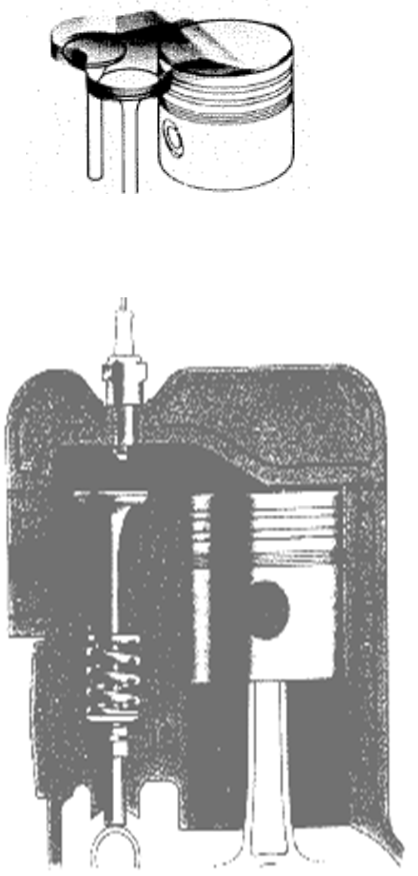
\includegraphics[scale=0.25]{ch4/20}
	\captionof{figure}{}
	\end{minipage}
	\begin{minipage}{0.18 \textwidth}
	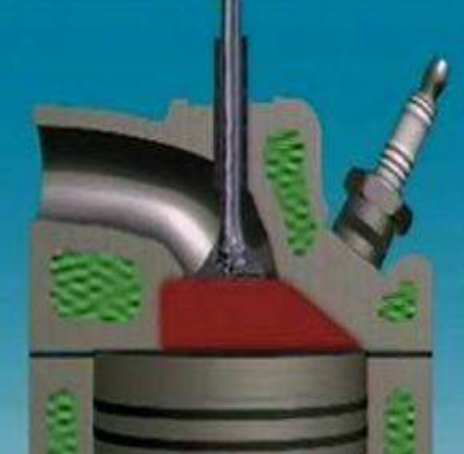
\includegraphics[scale=0.3]{ch4/21}
	\captionof{figure}{}
	\end{minipage}
	\begin{minipage}{0.18\textwidth}
	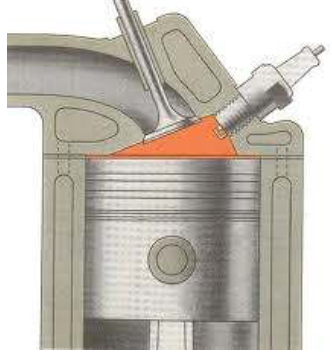
\includegraphics[scale=0.5]{ch4/22}
	\captionof{figure}{}
	\end{minipage}
	\begin{minipage}{0.18\textwidth}
	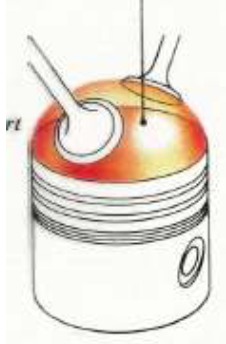
\includegraphics[scale=0.5]{ch4/23}
	\captionof{figure}{}
	\end{minipage}
	\begin{minipage}{0.18 \textwidth}
	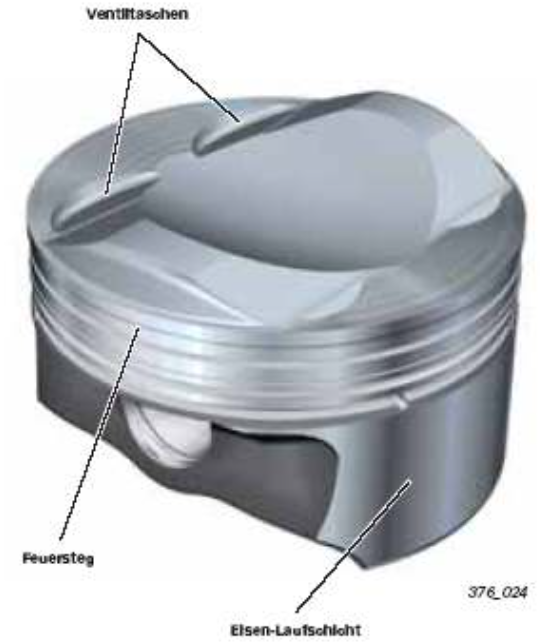
\includegraphics[scale=0.25]{ch4/24}
	\captionof{figure}{}
	\end{minipage}
	\end{center}
	
	\paragraph{Side valve engine}
	Simple construction, but the valve is aside the piston, the distance from the spark to the cylinder walls is larger and the combustion chamber is small, so this design is more sensitive to knocks. We will lower the compression ratio, but this is not good for the efficiency. 
	
	\paragraph{Bath tub shaped}
	Short flame distance to the wall, enough turbulence caused by the long oval side and the mixture is compressed in the cylinder head. 
	
	\paragraph{Wedge-shaped}
	Short distance and good whirl since the air is pushed from spark plug to the other side. 
	
	\paragraph{Hemispherical}
	Good distance to the walls, large space for the valves and good cooling. 
	
	\paragraph{Directly injected engines}
	Combination of a roof shaped combustion chamber with a shaped piston, turbulent mixture is pushed to the spark. 